\documentclass[]{standalone}
\usepackage[dvipsnames]{xcolor}
\usepackage{tikz-network}
\begin{document}
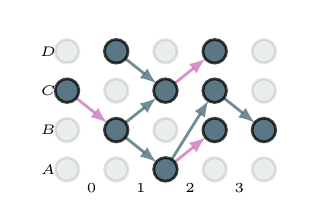
\begin{tikzpicture}
    \pgfmathsetmacro{\width}{2.5}
    \pgfmathsetmacro{\height}{1.5}
    \pgfmathsetmacro{\margin}{0.5 + 0.2}
    \tikzset{every node}=[font=\sffamily\bfseries]
    \clip (-\margin*\width cm,-\margin*\height cm) rectangle (\margin*\width cm,\margin*\height cm);
    \draw[draw,opacity=0] (-\margin*\width cm,-\margin*\height cm) rectangle (\margin*\width cm,\margin*\height cm);
    \Vertex[RGB,color={36, 74, 92},size=0.3,opacity=0.1,style={draw opacity=0.1},x=-1.25,y=-0.75]{A0};
\Vertex[RGB,color={36, 74, 92},size=0.3,opacity=0.1,style={draw opacity=0.1},x=-0.625,y=-0.75]{A1};
\Vertex[RGB,color={36, 74, 92},size=0.3,opacity=0.75,style={draw opacity=0.75},x=0.0,y=-0.75]{A2};
\Vertex[RGB,color={36, 74, 92},size=0.3,opacity=0.1,style={draw opacity=0.1},x=0.625,y=-0.75]{A3};
\Vertex[RGB,color={36, 74, 92},size=0.3,opacity=0.1,style={draw opacity=0.1},x=1.25,y=-0.75]{A4};
\Vertex[RGB,color={36, 74, 92},size=0.3,opacity=0.1,style={draw opacity=0.1},x=-1.25,y=-0.25]{B0};
\Vertex[RGB,color={36, 74, 92},size=0.3,opacity=0.75,style={draw opacity=0.75},x=-0.625,y=-0.25]{B1};
\Vertex[RGB,color={36, 74, 92},size=0.3,opacity=0.1,style={draw opacity=0.1},x=0.0,y=-0.25]{B2};
\Vertex[RGB,color={36, 74, 92},size=0.3,opacity=0.75,style={draw opacity=0.75},x=0.625,y=-0.25]{B3};
\Vertex[RGB,color={36, 74, 92},size=0.3,opacity=0.75,style={draw opacity=0.75},x=1.25,y=-0.25]{B4};
\Vertex[RGB,color={36, 74, 92},size=0.3,opacity=0.75,style={draw opacity=0.75},x=-1.25,y=0.24999999999999994]{C0};
\Vertex[RGB,color={36, 74, 92},size=0.3,opacity=0.1,style={draw opacity=0.1},x=-0.625,y=0.24999999999999994]{C1};
\Vertex[RGB,color={36, 74, 92},size=0.3,opacity=0.75,style={draw opacity=0.75},x=0.0,y=0.24999999999999994]{C2};
\Vertex[RGB,color={36, 74, 92},size=0.3,opacity=0.75,style={draw opacity=0.75},x=0.625,y=0.24999999999999994]{C3};
\Vertex[RGB,color={36, 74, 92},size=0.3,opacity=0.1,style={draw opacity=0.1},x=1.25,y=0.24999999999999994]{C4};
\Vertex[RGB,color={36, 74, 92},size=0.3,opacity=0.1,style={draw opacity=0.1},x=-1.25,y=0.75]{D0};
\Vertex[RGB,color={36, 74, 92},size=0.3,opacity=0.75,style={draw opacity=0.75},x=-0.625,y=0.75]{D1};
\Vertex[RGB,color={36, 74, 92},size=0.3,opacity=0.1,style={draw opacity=0.1},x=0.0,y=0.75]{D2};
\Vertex[RGB,color={36, 74, 92},size=0.3,opacity=0.75,style={draw opacity=0.75},x=0.625,y=0.75]{D3};
\Vertex[RGB,color={36, 74, 92},size=0.3,opacity=0.1,style={draw opacity=0.1},x=1.25,y=0.75]{D4};
\Vertex[label=$A$,fontsize=\fontsize{4}{10}\selectfont,opacity=0.0,style={draw=none},x=-1.49,y=-0.75]{label_A};
\Vertex[label=$B$,fontsize=\fontsize{4}{10}\selectfont,opacity=0.0,style={draw=none},x=-1.49,y=-0.25]{label_B};
\Vertex[label=$C$,fontsize=\fontsize{4}{10}\selectfont,opacity=0.0,style={draw=none},x=-1.49,y=0.24999999999999994]{label_C};
\Vertex[label=$D$,fontsize=\fontsize{4}{10}\selectfont,opacity=0.0,style={draw=none},x=-1.49,y=0.75]{label_D};
\Vertex[label=$0$,fontsize=\fontsize{4}{10}\selectfont,opacity=0.0,style={draw=none},x=-0.9375,y=-0.99]{time_A};
\Vertex[label=$1$,fontsize=\fontsize{4}{10}\selectfont,opacity=0.0,style={draw=none},x=-0.3125,y=-0.99]{time_A};
\Vertex[label=$2$,fontsize=\fontsize{4}{10}\selectfont,opacity=0.0,style={draw=none},x=0.3125,y=-0.99]{time_A};
\Vertex[label=$3$,fontsize=\fontsize{4}{10}\selectfont,opacity=0.0,style={draw=none},x=0.9375,y=-0.99]{time_A};
\Edge[Direct,RGB,color={204, 120, 188},lw=1,opacity=0.8](C0)(B1);
\Edge[Direct,RGB,color={76, 112, 123},lw=1,opacity=0.8](B1)(C2);
\Edge[Direct,RGB,color={76, 112, 123},lw=1,opacity=0.8](B1)(A2);
\Edge[Direct,RGB,color={76, 112, 123},lw=1,opacity=0.8](D1)(C2);
\Edge[Direct,RGB,color={204, 120, 188},lw=1,opacity=0.8](A2)(B3);
\Edge[Direct,RGB,color={76, 112, 123},lw=1,opacity=0.8](A2)(C3);
\Edge[Direct,RGB,color={204, 120, 188},lw=1,opacity=0.8](C2)(D3);
\Edge[Direct,RGB,color={76, 112, 123},lw=1,opacity=0.8](C3)(B4);

\end{tikzpicture}
\end{document}
